\chapter{Packet Headers and Formats}
\label{chap:pformat}

The procedures and functions described in this chapter can be found in
\nsf{tcl/lib/ns-lib.tcl},
\nsf{tcl/lib/ns-packet.tcl}, and \nsf{packet.\{cc, h\}}.

Objects in the \clsref{Packet}{../ns-2/packets.h} are the fundamental unit of
exchange between objects in the simulation.
The class \code{Packet}
provides enough information to link a packet on to a list
(\ie, in a \code{PacketQueue} or on a free list of packets),
refer to a buffer containing packet headers
that are defined on a per-protocol basis,
and to refer to a buffer of packet data.
New protocols may define their own packet headers or may extend
existing headers with additional fields.

New packet headers are introduced into the simulator
by defining a C++ structure with the needed fields,
defining a static class to provide OTcl linkage,
and then modifying some of the simulator initialization code
to assign a byte offset in each packet where the new header
is to be located relative to others.

When the simulator is initialized through OTcl,
a user may choose to enable
only a subset of the compiled-in packet formats, resulting in
a modest savings of memory during the execution of the simulation.
Presently, most configured-in packet formats are enabled.
The management of which packet formats are currently enabled
in a simulation is handled by a special packet header manager
object described below.
This object supports an OTcl method used to specify
which packet headers will be used in a simulation.
If an object in the simulator makes use of a field in a header
which has not been enabled, a run-time fatal program abort occurs.

\section{A Protocol-Specific Packet Header}
\label{sec:ppackethdr}

Protocol developers
will often wish to provide a specific header type to be used in packets.
Doing so allows a new protocol implementation
to avoid overloading already-existing header fields.
We consider a simplified version of RTP as an example.
The RTP header will require a sequence number fields and a source
identifier field.
The following classes create the needed header
(see \nsf{rtp.h} and \nsf{rtp.cc}):
\begin{program}
{\rm From rtp.h:}
        /* {\cf rtp packet.  For now, just have srcid + seqno.} */
        struct hdr_rtp \{ 
                u_int32_t srcid_;
                int seqno_;
                /* {\cf per-field member functions } */
                u_int32_t& srcid() \{ return (srcid_); \}
                int& seqno() \{ return (seqno_); \}

                /* {\cf Packet header access functions} */
                static int offset_;
                inline static int& offset() \{ return offset_; \}
                inline static hdr_rtp* access(const Packet* p) \{
                        return (hdr_rtp*) p->access(offset_);
                \}
        \};

{\rm From rtp.cc:}

        class RTPHeaderClass : public PacketHeaderClass \{
        public: 
                RTPHeaderClass() : PacketHeaderClass("PacketHeader/RTP",
                                                     sizeof(hdr_rtp)) \{
                        bind_offset(&hdr_rtp::offset_);
                \}
        \} class_rtphdr;

        void RTPAgent::sendpkt()
        \{
                Packet* p = allocpkt();
                hdr_rtp *rh = hdr_rtp::access(p);
                lastpkttime_ = Scheduler::instance().clock();

                /* {\cf Fill in srcid_ and seqno} */
                rh->seqno() = seqno_++;
                rh->srcid() = session_->srcid();
                target_->recv(p, 0);
        \}

        RTPAgent::RTPAgent()
                : session_(0), lastpkttime_(-1e6)
        \{
                type_ = PT_RTP;
                bind("seqno_", &seqno_);
        \}
\end{program}
The first structure, \code{hdr_rtp}, defines the layout
of the RTP packet header (in terms of words and their placement):
which fields are needed and how big they are.
This structure definition is only used by the
compiler to compute byte offsets of fields;
no objects of this structure type are ever directly allocated.
The structure also provides member functions which in turn
provide a layer of data hiding for objects wishing to read
or modify header fields of packets.
Note that the static class variable \code{offset_} is used
to find the byte offset at which the rtp header is located
in an arbitrary \ns packet.
Two methods are provided to utilize this variable to access this
header in any packet: \code{offset()} and \code{access()}.
The latter is what most users should choose to access this particular
header in a packet; the former is used by the packet header management
class and should seldom be used.
For example, to access the RTP packet header in a packet pointed by
\code{p}, one simply says \code{hdr_rtp::access(p)}.
The actual binding of \code{offset_} to the position of this header in
a packet is done by routines inside \nsf{tcl/lib/ns-packet.tcl} and
\nsf{packet.cc}.
The \code{const} in \code{access()}'s argument provides (presumably)
read-only access to a \code{const} Packet, lthough read-only is
enforced since the return pointer is not \code{const}. 
One correct way to do this is to provide two methods, one for write
access, the other for read-only access.
However, this is not currently implemented.

{\bf IMPORTANT}: Notice that this is completely different from the
{\em original} (and obsolete) method to access a packet header, which
requires that an 
integer variable, \code{off_\tup{hdrname}_}, be defined for any packet
header that one needs to access.
This method is now obsolete; its usage is tricky and its misuse can
be very difficult to detect. 

% which is accomplished by declaring and binding the integer variable
% \code{off_\tup{hdrname}_}
% where \code{\tup{hdrname}} refers to a shorthand name
% of the header of interest which must match the
% name assigned in \nsf{tcl/lib/ns-packet.tcl}.
% This is performed above by the RTPAgent's constructor.
% Generally, one header object for each type of header
% in the simulation is instantiated at simulator run-time.
% A particular header is enabled via OTcl in the simulation during
% simulator configuration time (see Section~\ref{sec:configpacket}).

The static object \code{class_rtphdr} of
\clsref{RTPHeaderClass}{../ns-2/rtp.cc} 
is used to provide linkage to OTcl when the RTP header is
enabled at configuration time.
When the simulator executes, this static object calls
the \code{PacketHeaderClass} constructor with arguments
\code{"PacketHeader/RTP"} and \code{sizeof(hdr_rtp)}.
This causes the size of the RTP header to be stored
and made available to the packet header manager
at configuration time (see below, Section~\ref{sec:packethdrmgr}).
Notice that \code{bind_offset()} {\bf MUST} be called in the 
constructor of this class, so that the packet
header manager knows where to store the offset for this particular
packet header. 

The sample member function \fcn[]{sendpkt} method
of \code{RTPAgent} creates a new packet
to send by calling \fcn[]{allocpkt}, which handles assignment
of all the network-layer packet header fields (in this case, IP).
Headers other than IP are handled separately.
In this case, the agent uses the \code{RTPHeader} defined above.
The \fcn{Packet::access} member function returns the address
of the first byte in a buffer used to hold header information (see below).
Its return value is cast as a pointer to the header of interest,
after which member functions of the \code{RTPHeader}
object are used to access individual fields.

\subsection{Adding a New Packet Header Type}

Assuming we wish to create a new header called \code{newhdr}
the following steps are performed:
\begin{enumerate}\itemsep0pt
  \item create a new structure defining the raw fields
        (called \code{hdr_newhdr}), define \code{offset_} and access
        methods. 
  \item define member functions for needed fields.
  \item create a static class to perform OTcl linkage
        (defines \code{PacketHeader/Newhdr}), do \code{bind_offset()}
        in its constructor. 
  \item edit \nsf{tcl/lib/ns-packet.tcl} to enable new packet format
        (see \ref{sec:pinfoclass}, \ref{sec:configpacket}).
\end{enumerate}

{\em This is the recommended way to add your packet headers. 
  If you do
  not follow this method, your simulation may still work, but it may 
  behave in a unpredictable way when more protocols are added into
  your simulation. 
  The reason is that the BOB (Bag of Bits,
  Section~\ref{sec:packetclass}) in \ns packet is a large
  sparse space, assigning one wrong packet header offset may not
  trigger failure immediately.}

\subsection{Selectively Including Packet Headers in Your Simulation}

By default, ns includes {\em ALL} packet headers of {\em ALL}
protocols in ns in {\em EVERY} packet in your simulation. 
This is a LOT of overhead, and will increase as more
protocols are added into ns.
For ``packet-intensive'' simulations, this could be a huge overhead.
For instance, as of now (Aug 30, 2000), the size of packet headers of
all protocols in ns is about 1.9KB; however, if you turn on only the
common header, the IP header and the TCP header, they add up to about
100 bytes. 
If you are doing large-scale web traffic simulation with many big fat
pipes, reducing unused packet headers can lead to major memory
saving.

To include only the packet headers that are of interest to you in your 
specific simulation, follow this pattern (e.g., you want to remove AODV
and ARP headers from your simulation):
\begin{program}
        remove-packet-header AODV ARP
        ......
        set ns [new Simulator]
\end{program}
Notice that \code{remove-packet-header} MUST go before the simulator
is created.
All packet header names are in the forms of
\code{PacketHeader/[hdr]}. 
You only need to supply the \code{[hdr]} part, not the prefix.
To find the names of packet headers, you may either look them up in 
\nsf{tcl/lib/ns-packet.tcl}, or run the following simple commands in
\ns: 
\begin{program}
        foreach cl [PacketHeader info subclass] \{
                puts $cl
        \}
\end{program} %$

To include only a specific set of headers in your simulation, e.g., IP
and TCP, follow this pattern:
\begin{program}
        remove-all-packet-headers
        add-packet-header IP TCP
        ......
        set ns [new Simulator]
\end{program}
IMPORTANT: You MUST never remove common header from your
simulation. 
As you can see in \nsf{tcl/lib/ns-packet.tcl}, this is enforced
by these header manipulation procs.

{\em Notice that by default, all packet headers are included}.

\section{Packet Classes}
\label{sec:packetclasses}

There are four C++ classes relevant to the handling of packets
and packet headers in general: \code{Packet}, \code{p_info}
\code{PacketHeader}, and \code{PacketHeaderManager}.
The \clsref{Packet}{../ns-2/packet.h}
defines the type for all packets in the simulation;
it is a subclass of \code{Event} so that packets may
be scheduled (e.g.~for later arrival at some queue).
The \clsref{packet\_info}{../ns-2/packet.h} holds all text
representations for packet names.
The \clsref{PacketHeader}{../ns-2/packet.h} provides a base class for
any packet header configured into the simulation.
It essentially provides 
enough internal state to locate any particular packet
header in the collection of packet headers present in any given packet.
The \clsref{PacketHeaderManager}{../ns-2/packet.h}
defines a class used to collect and manage currently-configured headers.
It is invoked by a method available to OTcl at simulation configuration
time to enable some subset of the compiled-in packet headers.

\subsection{The Packet Class}
\label{sec:packetclass}

The class Packet defines the structure of a
packet and provides member functions to handle a
free list for objects of this type.
It is illustrated in Figure~\ref{pic:packet} and
defined as follows in \code{packet.h}:
\begin{figure}[h]
  \centerline{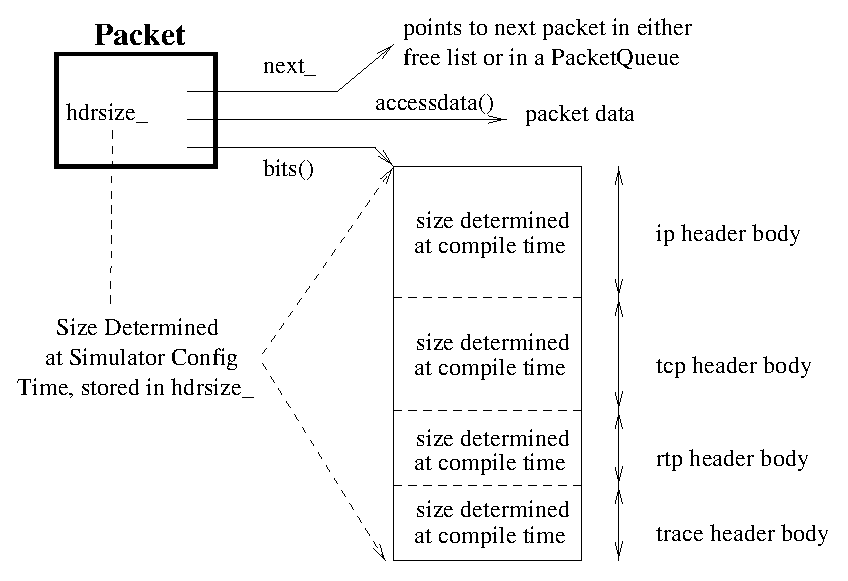
\includegraphics{packet}}
  \caption{A Packet Object}
  \label{pic:packet}
\end{figure}
\begin{program}
        class Packet : public Event \{
        private:
                friend class PacketQueue;
                u_char* bits_;  
                u_char* data_;  \* variable size buffer for 'data' */
                u_int datalen_; \* length of variable size buffer */
        protected:
                static Packet* free_;
        public: 
                Packet* next_;  \* for queues and the free list */
                static int hdrlen_;
                Packet() : bits_(0), datalen_(0), next_(0) \{\}
                u_char* const bits() \{ return (bits_); \}
                Packet* copy() const;
                static Packet* alloc();
                static Packet* alloc(int);
                inline void allocdata(int);
                static void free(Packet*);
                inline u_char* access(int off) \{
                        if (off < 0)
                                abort();
                        return (&bits_[off]);
                \}  
                inline u_char* accessdata() \{ return data_; \}
        \};
\end{program}
This class holds a pointer to a generic array of unsigned
characters (commonly called the ``bag of bits'' or BOB for short)
where packet header fields are stored.
It also holds a pointer to packet ``data'' (which is often not used in
simulations).
The \code{bits_} variable contains the address of
the first byte of the BOB.
Effectively BOB is (currently implemented as) a concatenation
of all the structures defined for each packet header (by convention,
the structures with names beginning \code{hdr_\tup{something}}) that have
been configured in.
BOB generally remains a fixed size throughout a simulation, and
the size is recorded in the \code{Packet::hdrlen_} member
variable.
This size is updated during simulator configuration by
OTcl\footnote{It is not intended to be updated after configuration
time.  Doing so {\em should} be possible, but is currently untested.}.

The other methods of the class Packet are for creating new
packets and storing old (unused) ones on a private free list.
Such allocation and deallocation is performed by the
following code (in \nsf{packet.h}):
\begin{program}
        inline Packet* Packet::alloc()
        \{
                Packet* p = free_;
                if (p != 0)
                        free_ = p->next_;
                else \{
                        p = new Packet;
                        p->bits_ = new u_char[hdrsize_];
                        if (p == 0 || p->bits_ == 0)
                                abort();
                \}
                return (p);
        \}

        /* {\cf allocate a packet with an n byte data buffer} */
        inline Packet* Packet::alloc(int n)
        \{
                Packet* p = alloc();
                if (n > 0)
                       p->allocdata(n);
                return (p);
        \}
                
        /* {\cf allocate an n byte data buffer to an existing packet} */
        inline void Packet::allocdata(int n)
        \{       
                datalen_ = n; 
                data_ = new u_char[n];
                if (data_ == 0)
                        abort();
         
        \}       

        inline void Packet::free(Packet* p)
        \{
                p->next_ = free_;
                free_ = p;
                if (p->datalen_) \{
                        delete p->data_;
                        p->datalen_ = 0;
                \}
        \}       
         
        inline Packet* Packet::copy() const
        \{               
                Packet* p = alloc();
                memcpy(p->bits(), bits_, hdrlen_);  
                if (datalen_) \{ 
                        p->datalen_ = datalen_;
                        p->data_ = new u_char[datalen_];
                        memcpy(p->data_, data_, datalen_);
                \}
                return (p);
        \}
\end{program}
The \fcn[]{alloc} method is a support function commonly
used to create new packets.
It is called by \fcn[]{Agent::allocpkt} method on
behalf of agents and is thus not normally invoked directly by most objects.
It first attempts to locate an old packet on the free list and
if this fails allocates a new one using the C++ \code{new} operator.
Note that \code{Packet} class objects and BOBs are
allocated separately.
The \fcn[]{free} method frees a packet by returning it to the free
list.
Note that \emph{packets are never returned to the system's memory allocator}.
Instead, they are stored on a free list when \fcn[]{Packet::free} is called.
The \fcn[]{copy} member creates a new, identical copy of a packet
with the exception of the \code{uid_} field, which is unique.
This function is used by \code{Replicator} objects to support
multicast distribution and LANs.

\subsection{p\_info Class}
\label{sec:pinfoclass}

This class is used as a ``glue'' to bind numeric packet type values
with their symbolic names.  When a new packet type is defined, its
numeric code should be added to the enumeration \code{packet_t} (see
\nsf{packet.h}) \footnote{Note: \code{PT\_NTYPE} should remain the last element of this
enumeration.} and its symbolic name should be added to the constructor
of \code{p_info}:
\begin{program}
enum packet_t \{
        PT_TCP,
        ...
        PT_NTYPE // This MUST be the LAST one
\};

class p_info \{
public:
        p_info() \{
                name_[PT_TCP]= "tcp";
                ...
        \}
\}
\end{program}
\subsection{The hdr\_cmn Class}
\label{sec:commonhdr}

Every packet in the simulator has a ``common''
header which is defined in \nsf{packet.h} as follows:
\begin{program}
        struct hdr_cmn \{
                double    ts_;            \* timestamp: for q-delay measurement */
                packet_t  ptype_;         \* packet type (see above) */
                int       uid_;           \* unique id */
                int       size_;          \* simulated packet size */
                int       iface_;         \* receiving interface (label) */
         
                /* {\cf Packet header access functions} */
                static int offset_;
                inline static int& offset() \{ return offset_; \}
                inline static hdr_cmn* access(Packet* p) \{
                        return (hdr_cmn*) p->access(offset_);
                \}

                /* {\cf per-field member functions} */
                int& ptype() \{ return (ptype_); \}
                int& uid() \{ return (uid_); \}
                int& size() \{ return (size_); \}
                int& iface() \{ return (iface_); \}
                double& timestamp() \{ return (ts_); \}
        \};
\end{program}
This structure primarily defines fields used for tracing
the flow of packets or measuring other quantities.
The time stamp field is used to measure queuing delay
at switch nodes.
The \code{ptype_} field is used to identify the
type of packets, which makes reading traces simpler.
The \code{uid_} field is used by the scheduler in scheduling
packet arrivals.
The \code{size_} field is of general use and gives the
simulated packet's size in bytes.
Note that the actual number of bytes consumed in the simulation
may not relate to the value of this field
  (i.e., \code{size_} has \emph{no} relationship
  to \code{sizeof(struct hdr_cmn)} or other ns structures).
Rather, it is used most often in computing the time required for a packet
to be delivered along a network link.
As such it should be set to the sum of the
  application data size
  and IP-, transport-, and application-level headers
  for the simulated packet.
The \code{iface_} field is used by the simulator when performing
multicast distribution tree computations.
It is a label indicating (typically) on which link a packet was received.

\subsection{The PacketHeaderManager Class}
\label{sec:packethdrmgr}

An object of the \clsref{PacketHeaderManager}{../ns-2/packet.h} is used
to manage the set of currently-active packet header types and
assign each of them unique offsets in the BOB.
It is defined in both the C++ and OTcl code:
\begin{program}
{\rm From tcl/lib/ns-packet.tcl:}
        PacketHeaderManager set hdrlen_ 0
        ......
        foreach prot \{
                AODV
                ARP
                aSRM 
                Common 
                CtrMcast 
                Diffusion
                ......
                TORA
                UMP 
        \} \{
                add-packet-header $prot
        \}
        Simulator instproc create_packetformat \{\} \{
                PacketHeaderManager instvar tab_
                set pm [new PacketHeaderManager]
                foreach cl [PacketHeader info subclass] \{
                        if [info exists tab_($cl)] \{
                                set off [$pm allochdr $cl]
                                $cl offset $off
                        \}
                \}
                $self set packetManager_ $pm
        \}
        PacketHeaderManager instproc allochdr cl \{
                set size [$cl set hdrlen_]
                $self instvar hdrlen_
                set NS_ALIGN 8 \; round up to nearest NS_ALIGN bytes, (needed on sparc/solaris);
                set incr [expr ($size + ($NS_ALIGN-1)) & ~($NS_ALIGN-1)]
                set base $hdrlen_
                incr hdrlen_ $incr
                return $base
        \}

{\rm From packet.cc:}
        /* {\cf manages active packet header types} */
        class PacketHeaderManager : public TclObject \{
        public:
                PacketHeaderManager() \{
                        bind("hdrlen_", &Packet::hdrlen_);
                \}
        \};
\end{program} %$
The code in \nsf{tcl/lib/ns-packet.tcl} is executed
when the simulator initializes.
Thus, the {\tt foreach} statement is executed before the
simulation begins, and initializes the OTcl class array
\code{tab_} to contain the mapping between class
the name and the names of the currently active packet header classes.
As discussed above (\ref{sec:ppackethdr}), packet headers should
be accessed using \code{hdr_\tup{hdrname}::access()}. 

The \proc[]{create\_packetformat} instance procedure is part of the
basic Simulator class and is called one time during simulator
configuration.
It first creates a single \code{PacketHeaderManager} object.
The C++ constructor links the OTcl instance
variable \code{hdrlen_} (of class \code{PacketHeaderManager})
to the C++ variable \code{Packet::hdrlen_} (a static
member of the \code{Packet} class).
This has the effect of setting \code{Packet::hdrlen_} to
zero.
Note that binding across class types in this fashion is
unusual.

\label{sec:configpacket}
After creating the packet manager, the \code{foreach}
loop enables each of the packet headers of interest.
This loop iterates through the list of defined
packet headers of the form
$(h_i, o_i)$ where $h_i$ is the name of the  $i$th header
and $o_i$ is the name of the variable containing the
location of the $h_i$ header in BOB.
The placement of headers is performed by the \code{allochdr}
instproc of the \code{PacketHeaderManager} OTcl class.
The procedure keeps a running variable \code{hdrlen_} with
the current length of BOB as new packet headers are enabled.
It also arranges for 8-byte alignment for any newly-enabled packet
header.
This is needed to ensure that when double-world length quantities
are used in packet headers on machines where double-word alignment
is required, access faults are not produced.\footnote{In
some processer architectures, including the
Sparc and HP-PA, double-word access must be performed on a double-word
boundary (i.e. addresses ending in 0 mod 8).  Attempting to perform
unaligned accesses result in an abnormal program termination.}.


\section{Commands at a glance}
\label{sec:pktcommand}

Following is a list of packet-header related procedures:
\begin{flushleft}
\code{Simulator::create_packetformat}

This is an internal simulator procedure and is called once during the simulator
configuration to setup a packetHeaderManager object.

\code{PacketHeaderManager::allochdr}

This is another internal procedure of Class PacketHeaderManager that
keeps track 
of a variable called \code{hdrlen_} as new packet-headers are
enabled. 
It also allows 8-byte allignment for any newly-enabled pkt header.

\code{add-packet-header}
takes a list of arguments, each of which is a packet header name
(without \code{PacketHeader/} prefix). This global proc will tell
simulator to include the specified packet header(s) in your
simulation. 
\code{remove-packet-header} operates in the same syntax, but it
removes the specified headers from your simulation; notice that it
does not remove the common header even it is instructed to do so.

\code{remove-all-packet-headers} is a global Tcl proc. It takes no
argument and removes all packet headers, except the common header,
from your simulation. \code{add-all-packet-headers} is its
counterpart. 

\end{flushleft}
\endinput
